\section{Introduction} \label{sec: intro}
\quad \quad 
With all of the different types of data that can come from a variety of sources, it is in today's market
to have a unified logging layer to sort and export all these different data sources. On the market, some
of the tools that can accomplish this tend to be on the expensive side, but there are also open source tools that
work to compete with these tools. One such tool is Fluentd, which is an unified logging layer that is comparable to
Logstash, another popular logging tool. Both of these tools can be connected to Kibana and the Elastic Stack, 
making them powerful logging tools when used correctly. The rest of the paper is structured as follows. The 
\hyperref[sec:motiv]{next section} gives the motivation as to why logging tools are important. 
\hyperref[sec:works]{Section 3} goes into more detail on how fluentd works under the hood, and also gives some
use cases. \hyperref[sec:comp]{Section 4} gives a comparison between the two popular logging layer tools, Logstash 
and Fluentd, as well as discuss how both connect the the ELK Stack. \hyperref[sec:demo]{Section 5} will give a demo on how to 
utilize Fluentd in different logging scenarios, and then \hyperref[sec:conclude]{section 6} will conclude the paper.
\section{Motivation} \label{sec:motiv}
\quad \quad 
Logging tools are important due to the structure and organization they can provide to data on a day to 
day basis. For example, if a company has multiple machines running applications and other programs, it would be nice 
to have all the log data of all the machines centralized in a single logging server. Tools like fluentd can do this, as 
they provide features for listening and filtering logs as they are created (more on how this works in the next section). 
In short, there are a variety of different logging tools out that have different functionalities and purposes. The two tools
that will be discussed in this paper, Fluentd and Logstash, are known for their ability to be unified logging layers that can
listen for and send data to a variety of destinations. Organization can be key when it comes to security and other subjects,
as there are some things that can only be seen when data has been brought together into one place and compared.
\section{How Fluentd Works} \label{sec:works}
\quad \quad 
At its most basic level, Fluentd is an unified logging layer that can take input from many different
data sources and route them to different sources depending on how a fluentd configuration file is formatted. Below is a chart
from the Fluentd website that shows how different data sources can be mapped.
\begin{figure}[H]
    \centering
    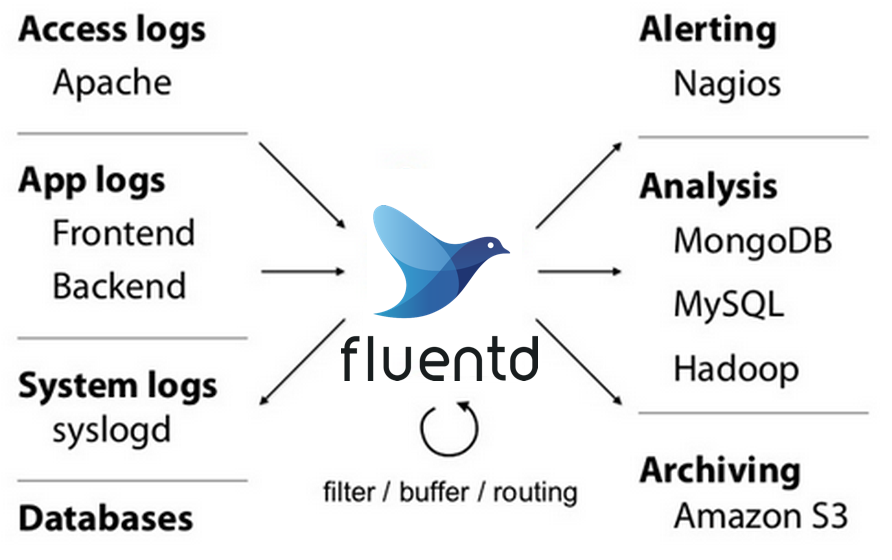
\includegraphics[scale=0.75]{images/fluentd-architecture.png}
    \caption{Fluentd Flow Diagram [2]}
    \label{fig:picture}
\end{figure}
With this you can easily route data to multiple different sources, or you could even route them to the same source if necessary.
This is done through a configuration file that can be easily modified with the following directives.
\subsection{The Source Directive}
\quad \quad The source directive is the part of the configuration file that \say{determine[s] the input of the sources}[1]. So within
the source directive, you can list the type of source you want to receive from, which can be anything ranging from a file, a TCP (transmission control protocl) packet,
a UDP (user datagram protocol) packet, or most importantly, a forward packet from another fluentd instance. With the last source mentioned in
particular, this allows multiple machine to link if they are each running a fluentd instance that can communicate with
each other.
\subsection{The Match Directive}
\quad \quad The match directive, opposite of the source directive, is a directive that \say{determine[s] the output destinations}[1]. Some possible output locations Fluentd 
send data to are a file, stdout (standard out), HTTP (hypertext transfer protocol) address, and more from installation. In order to forward data to
other services such as elasticsearch, kafka, mongoDB, and others it is necessary to do some extra installation for those output plugins. The installation for those services
listed never was too strenuous though, with the instructions listed only taking one to two command line instructions to install all the dependencies.
\subsection{The Filter Directive}
\quad \quad The filter directive is an unique directive that \say{determine[s] the event processing pipelines}[1]. What this means is that it can be used to alter a data stream
it goes through Fluentd. For example, a piece of data could come into fluentd via a source directive, go through a filter directive to add to the contents of that data stream, and
then finally go to through a match directive and get forwarded to the output destination of choice.
\subsection{Putting everything together}
\section{Fluentd and Logstash} \label{sec:comp}
\quad \quad
\section{Fluentd demo} \label{sec:demo}
\quad \quad 
\section{Conclusion} \label{sec:conclude}
\quad \quad 
\newpage
\begin{thebibliography}{widest entry}
    \bibitem{1}{Fluentd 1.0 Documentation. (2021). Fluentd. https://docs.fluentd.org/}
    \bibitem{2}{Fluentd Architecture Overview. (2021). What is Fluentd?. \\https://www.fluentd.org/architecture}
    \bibitem{3}{Platform9. (2020, February 11). Kubernetes Logging: Comparing Fluentd vs. Logstash. https://platform9.com/blog/kubernetes-logging-comparing-fluentd-vs-logstash/}
    \bibitem{4}{Reock, Justin. (2020, April 14). Fluentd vs Logstash: How to Decide for Your Organization. https://www.openlogic.com/blog/fluentd-vs-logstash}
    \bibitem{5}{Chelat, Ajit. (2021, April 9). Fluentd vs. Logstash: The Ultimate Log Agent Battle. https://www.logiq.ai/fluentd-vs-logstash-the-ultimate-log-battle/}
    \bibitem{6}{Docker docs. (2021). Fluentd logging driver. \\https://docs.docker.com/config/containers/logging/fluentd/}
\end{thebibliography}